% -*- mode: latex; mode: auto-fill; -*-
% -*- set-buffer-file-coding-system: utf-8; -*-

\subsection{The Eulerian and Lagrangian point of view}
% Through the report, the examples and theory will be presented in the
% 2D .. as this is easy to visualise on paper. After each of the
% describtions this will be extended to 3D, and all formules for the 3D
% calculations will be explicit written so the reader knows all the
% details which is later use to implement the simulation.

When descriping motion of a substance, no mather if it is on fluid
(gass or liquid) or solid state, we have two well known models which
captures the problem: the Eulerian and the Lagrangian viewpoints. To
understand the difference between to the viewpoints we imagine how we
could measure the movement of e.g. a fluid. In the Eulerian viewpoint
we would place measuring devices at fixed points in the fluid, and
continues sample the velocity of the fluid, the measured value is
taken as a avarage for an area. For conviniences the measuring devices
are almost always placed in a uniform grid, with square areas as
illustrated in figure \ref{fig:eulerian}.

\begin{figure}[h]
  \centering
  \subfloat[Eulerian]{
    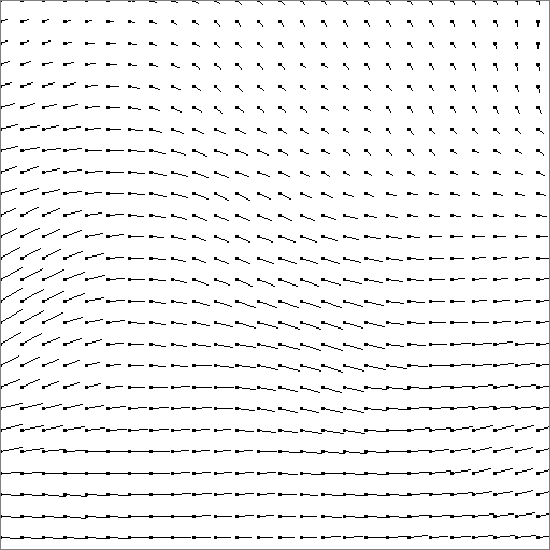
\includegraphics[width=0.5\textwidth]{imgs/eulerian.png}
    \label{fig:eulerian}
  }
  \subfloat[Lagrangian]{
    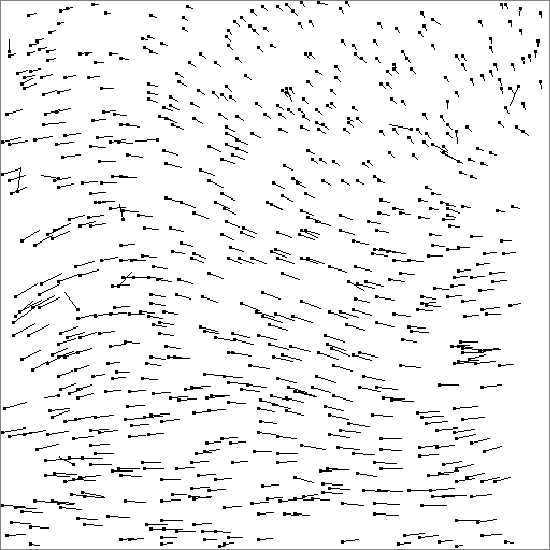
\includegraphics[width=0.5\textwidth]{imgs/lagrangian.png}
    \label{fig:lagrangian}
  }
  \caption{The eulerian and the lagrangian viewpoints.}
  \label{fig:eulerian-lagrangian}
\end{figure}

In the lagrangian viewpoint we let the measuring devices move along
the current in the fluid and take measurements at different locations
in the fluid. Here we imagen that the measuring device is part of the
fuild or a particle that the fluid moves around. Figure
\ref{fig:lagrangian} shows how the current has moved the devices as
time has progressed.

These two viewpoints are tightly coupled to the way the simulation data
is represented and visuliazed. Lets say that we are interested in
visualizing the surface of the substance.
%
The Lagrangian data is keept as points in space and moved around by
updating the position of the points. This can be visualizes by
imposing that the points define a surface and rendered as geometry
e.g. triangles between the points.
%
The eulerian viewpoint is seen as a 3D grid. Each cell in the grid has
a density that describes how much substance the cell contains (0-100\%).

Whiled this example focuses on measuring movement, the two different
viewpoints can be imposed on all kinds measurements.
%
When modelling a fluid, the Eulerian viewpoint is often
enough. But for more advanced simulations of fluid or solid,
Lagrangian is often used so the underlaying math equations are simpler
to describe.

%And example of this is: When modelling ...

%The are algoritmens that converts between the two viewpoints: .. . And
%as such nothing prevents us from using both viewpoint when defining
%the mathematically models that drives the simulation. As can be seen
%from the conversion algorithms, this envolves a fair amount of
%math. So to make the models more readable, it is advised to model
%in one of the domains, and only when optimizing the formulaes for
%performance, introduce conversions.

%In all the mathematically models that are developed in this repor the
%Lagrangian viewpoint is will be used.

%ref: fluids book, michael bang figures,

% \subsection{Data models}
% In the different parts of the simulator we use two different data
% model which are coupled tightly the the two points of view just
% reviewed. The two data models are refered to as the vertex/primitive
% model and the volumetric model. Each of which will now be elaborated.

% \subsubsection{The Vertex/Primitive model}
% When using the Lagragian viewpoint, we call the data model for a
% vertex/primitive model. In this model we have a vertex pool
% constituting which points are available, and some primitives, which
% referes to the vertices and binds these togther.

% \textbf{Primitives}
%  Fx as triangle, quads or tetrahedras.

% \subsubsection{The volumetric model}
% When using the Euler viewpoint in 2D, vi call the grid a texture and
% the cell for pixels. As we moves to 3D pixels are called voxels as
% they cover a volume.

% \textbf{density field}
% The voxels has value from 0 to 1. Which is to be interpreted as the
% procentage of solid the voxel contains.
% \textbf{Vector fields} \url{http://en.wikipedia.org/wiki/Vector_field}
% \textbf{Tensor fields} \url{http://en.wikipedia.org/wiki/Tensor_field}
% \textbf{energi density field}
% \url{http://users.powernet.co.uk/bearsoft/Field.html}

% \textbf{ISO Surface (level sets)}
% Each voxel is set to zero when it contains the surface of the solid
% and 1 all other places. \url{http://en.wikipedia.org/wiki/Isosurface}

% \textbf{distance field}
% Nearly the same as an iso surface. That is it zero on the surface, but
% instead of being 1 elseware, the voxels contains a value corresponding
% to the shortests distance to the surface.

% \textbf{signed distance field (SDF)}
% A distance field, but with a sign determining if the voxel is inside or
% outside the solid. So fx the distances inside the solid could be
% negative, and the voxels outside could be positive.

% The density field can be converted into a signed distance field or iso
% surface and rendered using standard volume rendering techniques.

% \subsubsection{Vertex/Primitive contra Volumetric}
% For a 3D graphics framework like OpenGL or DirectX, the
% vertex/primitive data model is the most convinient as data can be
% mapped directly to visual output.
% %
% But in some situations the vertex/primitive model is not the first
% choise. When representing the data as volumetric data the data model
% imposes a grid structure on the data, making some thing easier to
% do. Fx when doing collision detection the volumetric model has
% advantages.

% \subsection{Getting geometry input data}

% \subsubsection{X-ray images}
% The main source of surface and body (geometry) data comes from 3D X-ray
% image scans. X-ray images are volumetric data in black and white where
% each voxel has a value which describes the density in that voxel.
% When taking an X-ray image of bones or teeth, X-ray pulses are
% shot through the body with radiographic film behind. The bones or
% teeth absorb the most photons by the photoelectric process, because
% they are more electron-dense. The X-rays that do not get absorbed turn
% the photographic film from white to black, leaving a white shadow of
% bones and teeth on the film.

% \subsubsection{Segmentation}
% Patients are scanned and the dentist or other personal prepare
% the X-ray images for simulation by segmenting out the tooth that is to
% be operated upon in the simulator. As an example the segmentation can
% be done in the software ITK-Snap as showen in figure
% \ref{fig:itk-snap}, in the figure the red tooth has been segmented by
% first applying an automatic segmentation algorithm and afterwards rofly
% adapted by hand. The tooth segmented with green, has only been
% automaticly segmented, which also shows as the segmentation flows into
% the tooth next to it.

% \begin{figure}[H]
%   \centering
%   \includegraphics[width=14cm]{./images/itk-snap.png}
%   \caption{Segmentation in ITK-Snap.}
%   \label{fig:itk-snap}
% \end{figure}

% After the segmentation has taken place, the 3D image is exported, into
% a unsigned byte density field where voxels in the model (maked as red
% in the figure) get value 255, and voxels outside the model are set to
% 0. A guide of how to use ITK-Snap is provide in appendix \ref{guide:itk-snap}.

% \section{The simulator parts}
% The full simulator is made up of several different part or sub
% simulators. Each of the sub simulators does different things, and must
% therefore be designed specifictly for the job they need to handle. As
% mentioned in the introduction, we have identified the following
% different sub simulators. Now is that time to specify what they do and
% how we think it can be done.

% \subsection{Cutting tissue}
% As in: Virtual Reality
% Heart\footnote{\url{http://www.systematic.dk/om+os/innovation}}. I
% vertex based model and tools like knife and tweezers.

% \begin{figure}[H]
%   \centering
%   \includegraphics[width=14cm]{./images/heart-sim.png}
%   \caption{Screenshot from: The Heart Simulator.}
%   \label{fig:heart-sim}
% \end{figure}

% Picture from: \url{http://www.jespermosegaard.dk/Projects}

% \url{http://www.alexandra.dk/nyhedsbrev/to/05/november05/status_cavi.htm}
% \url{http://www.cavi.dk/projects/surgical_simulation.php}
% \url{http://www.daimi.au.dk/~mosegard/medVisSim/}
% \url{http://cg.alexandra.dk/2009/04/30/simulation-of-congenital-heart-surgery/}
% \url{http://www.daimi.au.dk/~cfpc/projects/cadiovas/cadiovas_summary.htm}

% \subsection{Dividing into smaller pieces}
% This job, has two distinct sub simulators, one for drilling and on for
% breaking. It has been divide this way, as the drilling is easiest done
% on a volumetric data model while the breaking is done using linear
% elastic model which are based on deforming the body making a vertex
% model more preferable.

% \subsubsection{Drilling}
% As the tooth have been segmented and exported from itk-snap, this data
% can be used directly in this sub simultor.
% %
% Drillng as done in the The Visible Ear
% Simulator\footnote{\url{http://www.alexandra.dk/ves/}}, are done
% directly on volumetric data. It works by simulating the drill head as
% a sphere, and when rotation the simulator modifies the voxels by
% removing material where the sphere are located.

% A possibility is to base the hardness of the material on the intensities
% of the material from the X-ray images.

% \begin{figure}[H]
%   \centering
%   \includegraphics[width=14cm]{./images/ear-sim.png}
%   \caption{Screenshot from: The Visible Ear Simulator.}
%   \label{fig:ear-sim}
% \end{figure}

% Picture taken from:
% \url{http://cg.alexandra.dk/category/visible-ear-simulator/}.

% To visualize the data, standard volumetric rendering techniques like
% ray tracing \ref{ray_tracing} or photon mapping \ref{photon_mapping}
% can be imployed. This is also what is done in The Visivle Ear
% Simulator.

% As all these techniques are implemented and used in The Visible Ear
% Simulator we can say for surtant that this is possible to simulate in
% real-time. But it is only possible because we do not need voxel models
% of the same magnitude as used in the ears simulator.

% \subsubsection{Breaking the tooth}
% As this sub simulator is the main topic of the thesis, it will be
% fulle described in the rest of the thesis. But to have an idear of
% what is to come this sub simulator models the tooth as a stiff
% material and tools for breaking the tooth are provided to the
% user. The model of the tooth uses triangles to model the surface
% and tetrahedrons for the body. We use the physics based elasticity
% theory and the finite element method to model deformation and
% energi. Lastly we employ fracture mechanics to model fracturing of the
% tooth when the energi raises above a limit defined for the material.

% \subsection{Removing pieces}
% This sub simulation is the least demanding simulation as all models
% in the sceen can be treated as ridig bodys, that is they cannot
% undergo deformation or other forms of modifications. They can only be
% move and rotated. So that main thing in this simulator is collision
% detection, which can be done naive on the GPU in real-time. The
% collision detection and tools needed here are very simulare to what is
% used in the heart simulation, and we are positive that this sub
% simulator will not be a problem to implement.

% \subsection{Stitching tissue}
% todo...

% \section{Binding the sub simulators together}
% Because the different sub simulator use different data models, we need
% to have a way of converting between the data models

% \subsection{Converting from Vertex/Primitive to Volumetric data}
% This convertion can be done by a algorithm known as flood filling.
% But to be able to use this algorithm the input model needs to be
% waterproof, meaning that the geometry must define a complete surface
% without any holes. A guide of how to do this convertion is provide in
% appendix \ref{guide:floodfilling}.

% \textbf{Generating Signed Distance Fields From Triangle Meshes}
% \url{http://citeseerx.ist.psu.edu/viewdoc/download?doi=10.1.1.111.6331&rep=rep1&type=pdf}

% \subsection{Converting from Volumetric to Vertex/Primitive data}
% This convertion can be done by a algorithm known as iso stuffing. ISO
% surface stuffing take a ISO surface as input, so to convert our
% density field we need to convert it to a ISO surface. A guide of how
% to do the density field to ISO surface converting and doing the ISO
% surface stuffing is provide in appendix \ref{guide:isosurfacestuffing}.

% \section{Hardware setup}
% Computer with monitor for visualisation, and some kind og haptic
% device for interacting with the simulator.

% \subsection{Haptic feedback}

% \begin{figure}[H]
%   \centering
%   \includegraphics[width=14cm]{./images/haptic_feedback.png}
%   \caption{Haptic feedback.}
%   \label{fig:haptic-feedback}
% \end{figure}

% \url{http://www.hjerteforeningen.dk/sw69890.asp}

%%% Local Variables: 
%%% mode: latex
%%% mode: auto-fill
%%% TeX-PDF-mode: t
%%% TeX-master: "../master.tex"
%%% End: 

